\documentclass[a4paper]{article}
\usepackage{header}
\begin{document}
\title{\LARGE{Алгоритмы и структуры данных—2}\\ Коллоквиум}
\author{Винер Даниил \href{https://t.me/danya_vin}{@danya\_vin}}
\date{Версия от \today}
\maketitle

% \section*{\LARGE{Алгоритмы и структуры данных—2. Коллоквиум}}
% \begin{flushright}
%     \textit{Основано на лекциях и тренировках}\\ 
%     \textit{по алгоритмам Михаила Густокашина}
% \end{flushright}
\tableofcontents
\newpage
\setlength{\parindent}{15pt}
\setlength{\parskip}{1.5mm} 
\section{Хэш-функция. Полиномиальное хэширование}
\subsection{Хэш-функция}
\definition Хэш-функцией называется функция, сопоставляющая объектам какого-то множества числовые значения из ограниченного промежутка.

\subsection{Полиномиальное хэширование}
Определим строку - как последовательность чисел от $1$ до $m$. Пусть $p=1e9+7$, или же любое другое огромное простое число, а также $k>m$.

Тогда, \textit{прямой полиномиальный хэш строки} есть значение такого многолена:
\begin{equation*}
    h_f=\left(s_0+s_1k+s_2k^2+\ldots+s_nk^n\right)\mod p
\end{equation*}
Или же, \textit{обратный полиномиальный хэш}:
\begin{equation*}
    h_b=\left(s_ok^n+s_1k^{n-1}+\ldots+s_n\right)\mod p
\end{equation*}

\difficulty $O(1)$, в таком случае мы поддерживаем переменную, равную нужной в данный момент степени $k$

\begin{lstlisting}
    const int k = 31, mod = 1e9+7;

    string s = "abacabadaba";
    long long h = 0, m = 1;
    for (char c : s) {
        int x = (int) (c - 'a' + 1);
        h = (h + m * x) % mod;
        m = (m * k) % mod;
    }

\end{lstlisting}

% \subsection{Идеальный хэш (Бонус от Вити)}
% \definition \textit{Идеальный хэш} — хэш, который без коллизий хэширует элементы за единицу врем



\subsection{Количество различных подстрок}   
Чтобы посчитать количество всех подстрок в строке длины $n$ нужно вычислить хэши всех подстрок и закинуть их в \code{set}. Тогда, \code{set.size()} — и будет количеством уникальных посдтрок в строке

\difficulty $O(n^2)$, где $n$ — длина строки, так как всего посдтрок $\displaystyle\frac{n(n+1)}{2}$

\subsection{Поиск подстроки в строке}
% Поиск реализуется с использованием алгоритма \textit{Рабина-Карпа}

Пусть $m$ — длина искомой подстроки. Для начала, вычисляем хэш искомой подстроки, назовем его \textit{эталонным}. После этого идем окном длины $m$ по всей строке, поддерживая хэш текущей подстроки. Если текущий хэш совпал с эталонным, то мы нашли подстроку

\difficulty $O(n)$, так как мы захэшируем всю строку, дл $n$
\subsection{Сравнения подстрок}
Для начала, создадим вектор \textit{баз}, который в дальнейшем поможет для полиномиального хэширования строки. Оптимально создать его так
\begin{lstlisting}
    int64_t mod = 1e9 + 7;
    base[0] = 1;
    for (size_t i = 1; i < base.size(); ++i) {
        base[i] = base[i - 1] * 257 % mod;
    }
\end{lstlisting}
Далее вычисляем массив префиксных хэшей, в котором $p_i$ — хэш строки от начала до $s_i$
\begin{lstlisting}
    std::vector<int64_t> p(s.size());
    for (size_t i = 1; i < p.size(); ++i) {
        p[i] = (p[i - 1] * base[1] + s[i]) % mod;
    }
\end{lstlisting}
После этого функция, вычисляющая хэш подстрок будет работать так: она принимает два индекса \code{i} и \code{j}. После этого вычисляем хэш предыдущей части строки, умноженный на соответствующую базу
\begin{lstlisting}
    int64_t hash(size_t i, size_t j){
        int64_t h = p[j] - p[i - 1] * base[j - i + 1] % mod;
        h = (mod + h) % mod;
        return h;
    }
\end{lstlisting}

\subsection{Палиндромность подстроки}
Можно посчитать два массива — обратные хэши и прямые. Проверка на палиндром будет заключаться в сравнении значений \code{hash\_substring()} на первом массиве и на втором.

\subsection{Количество палиндромов}
Можно перебрать центр палиндрома, а для каждого центра — бинпоиском его размер. Далее проверяем подстроку на палиндромность. Заметим, что случаи четных и нечетных палиндромов нужно обрабатывать отдельно

\begin{itemize}
    \item Перебираем каждый возможный центр (как для нечётных, так и для чётных палиндромов);
    \item Для каждого центра используем бинарный поиск, чтобы определить максимальный размер палиндрома;
    \item Проверяем, является ли подстрока палиндромом с помощью хешей;
    \item Считаем общее количество палиндромов
\end{itemize}

\newpage
\section{Z-функция. Префикс функция}
\subsection{Z-функция}
Z-функция от строки $s$ — массив $z$, такой что $z_i$ равно длине максимальной подстроки, начинающейся с $i$-й позиции, которая равна префиксу $s$

$$
\underbrace{aba}c\overbrace{aba}daba \hspace{1em} (z_4 = 3)
$$

\subsection{Построение z-функции за $O(n)$}
Будем идти слева направо и хранить \textit{z-блок} — самую правую подстроку, равную префиксу, которую мы успели обнаружить. Будем обозначать его границы как $l$ и $r$ включительно.

Пусть мы сейчас хотим найти $z_i$, а все предыдущие уже нашли. Новый $i$-й символ может лежать либо правее z-блока, либо внутри него:
\begin{itemize}
    \item Если правее, то мы просто наивно перебором найдем $z_i$ (максимальный отрезок, начинающийся с $s_i$ и равный префиксу), и объявим его новым z-блоком.
    \item Если $i$-й элемент лежит внутри z-блока, то мы можем посмотреть на значение $z_{i-l}$ и использовать его, чтобы инициализировать $z_i$ чем-то, возможно, отличным от нуля. Если $z_{i-l}$ левее правой границы $z$-блока, то $z_i = z_{i-l}$ — больше $z_i$ быть не может. Если он упирается в границу, то «обрежем» его до неё и будем увеличивать на единичку.
\end{itemize}

\begin{lstlisting}
    vector<int> z_function(string s) {
        int n = (int) s.size();
        vector<int> z(n, 0);
        int l = 0, r = 0;
        for (int i = 1; i < n; i++) {
            if (i <= r)
                z[i] = min(r - i + 1, z[i - l]);
            while (i + z[i] < n && s[z[i]] == s[i + z[i]])
                z[i]++;
            if (i + z[i] - 1 > r) {
                r = i + z[i] - 1;
                l = i;
            }
        }
        return z;
    }
\end{lstlisting}


\subsection{Префикс функция}
Префикс-функцией от строки $s$ называется массив $p$, где $p_i$ равно длине самого большого префикса строки $s_0 s_1 s_2 \ldots s_i$, который также является и суффиксом $i$-того префикса (не считая весь $i$-й префикс)

\subsection{Построение префикс функции за $O(n)$}

\begin{enumerate}
    \item \textbf{Инициализация}:
    \begin{itemize}
        \item Создаем массив $\pi$ длиной $N$ и инициализируем его нулями.
        \item Устанавливаем переменную $k = 0$, которая будет отслеживать длину текущего префикса.
    \end{itemize}

    \item \textbf{Итерация по строке}:
    \begin{itemize}
        \item Для каждого символа $s[i]$ от 1 до $N-1$:
        \begin{itemize}
            \item Если $s[i]$ совпадает с $s[k]$ (т.е. $s[i] == s[k]$):
            \begin{itemize}
                \item Увеличиваем $k$ на 1 и присваиваем $\pi[i] = k$.
            \end{itemize}
            \item Если они не совпадают:
            \begin{itemize}
                \item Пока $k > 0$ и $s[i]$ не совпадает с $s[k]$:
                \begin{itemize}
                    \item Обновляем $k$ с помощью $k = \pi[k-1]$.
                \end{itemize}
                \item После выхода из цикла, если $s[i]$ совпадает с $s[k]$, то снова увеличиваем $k$ и присваиваем $\pi[i] = k$.
                \item Если нет совпадений, оставляем $\pi[i] = 0$.
            \end{itemize}
        \end{itemize}
    \end{itemize}
\end{enumerate}

\subsection{Поиск подстроки в строке}
\subsubsection{Z-функцией}
Пусть у нас есть строка $s$ и паттерн $p$
\begin{itemize}
    % \item Совместим две эти строки в одну большую разделив символом \#
    \item Добавим к строке $s$ символ \#
    
    Можно взять любой другой символ, который гарантированно не встречается ни в $p$, ни в $s$ и имеет меньший ASCII-код, чем символы строки $s$. Получим
    % $$T=p+\#+s$$
    $$T=\#+s$$
    \item Теперь вычисляем для строки $T$ её Z-функцию
    \item После этого ищем в Z-функции все значения равные длине $p$. Если \code{z[i]=len(p)}, тогда подстрока $p$ начинается в строке $T$ с позиции $i$, а значит в строке $s$ — с позиции \code{i-len(p)-1}
\end{itemize}

% Можно взять любой другой символ, который гарантированно не встречается ни в $p$, ни в $s$ и имеет меньший ASCII-код, чем символы строки $s$. Получим
% $$T=p+\#+s$$

% Теперь вычисляем для строки $T$ ее Z-функцию. 
\subsubsection{Префикс-функцией}
Алгоритм похож на поиск подстроки с применением z-функций

Пусть дана строка $t$ и паттерн $s$. Составим строку $K=s+\#+t$. Пусть $n$ — длина строки $s$, а $m$ — строки $t$
\begin{enumerate}
    \item Считаем префикс-функцию для строки $K$
    \item Рассмотрим значения префикс-функции, кроме первых $n+1$, так как это строка $s$ и разделитель
    \begin{itemize}
        \item Если в какой-то позиции $i$ оказалось, что $\pi[i]=n$, то в позиции $i-(n+1)-n+1=i-2n$ строки $t$ начинается очередное вхождение паттерна
    \end{itemize}
\end{enumerate}

\subsubsection*{Почему это работает}
По определению, значение $\pi[i]$ — самая длинная подстрока, которая заканчивается в позиции $i$ и совпадает с префиксом

В нашем случае, $\pi[i]$ — фактически длина наибольшего блока совпадения со строкой $s$ и оканчивающегося в позиции $i$

Больше, чем $n$, эта длина быть не может — за счёт разделителя. Равенство $\pi[i] = n$, означает, что в позиции $i$ оканчивается искомое вхождение строки $s$

\difficulty $O(n+m)$


\subsection{Количество различных подстрок в строке}
\subsubsection{Z-функцией}
Дана строка $s$ длины $n$. Подсчет уникальных подстрок будем делать итеративно, то есть, зная текущее количество различных подстрок, пересчитывать это количество при добавлении в конец какого-то одного символа.

Пусть $k$ — текущее количество различных подстрок строки $s$, и мы добавляем в конец символ $c$
\begin{itemize}
    \item Возьмём строку $t = s + c$ и инвертируем её. Наша задача — посчитать, сколько у строки $t$ таких префиксов, которые не встречаются в ней более нигде
    \item Посчитаем Z-функцию для строки $t$ и найдём максимальное значение $z_{\rm max}$, тогда в строке $t$ встречается (не в начале) её префикс длины $z_{\rm max}$, но не большей длины. Понятно, префиксы меньшей длины уже точно встречаются в ней
\end{itemize}

Тогда, число новых подстрок, появляющихся при дописывании символа $c$, равно $len - z_{\rm max}$, где $len$ — длина строки \textbf{после приписывания символа} $c$.

\difficulty Для строки длины $n$ — $O(n^2)$

\ex Допустим, у нас есть строка $abacaba$ и мы хотим приписать в конец символ $k$. Тогда, посчитаем Z-функцию для строки $kabacaba$:
\begin{equation*}
    0,0,0,0,0,0,0,0
\end{equation*}
В данном случае, $z_{max}=0\Longrightarrow len-z_{max}=8$, то есть количество <<новых>> подстрок равно 8
% Аналогично можно пересчитывать за $O(n)$ количество различных подстрок и при дописывании символа в начало, а также при удалении символа с конца или с начала.


\subsubsection{Префикс-функцией}
Алгоритм практически идентичен алгоритму определения количества подстрок с помощью z-функции
\begin{itemize}
    \item Возьмём строку $t = s + c$ и инвертируем её. Наша задача — посчитать, сколько у строки $t$ таких префиксов, которые не встречаются в ней более нигде
    \item Если мы посчитаем для строки $t$ префикс-функцию и найдём её максимальное значение $\pi_{\rm max}$, то, очевидно, в строке $t$ встречается (не в начале) её префикс длины $\pi_{\rm max}$, но не большей длины
\end{itemize}

Тогда, число новых подстрок, появляющихся при дописывании символа $c$, равно 
$$s.size() + 1 - \pi_{\rm max}$$

\difficulty Для каждого дописываемого символа мы за $O(n)$ можем пересчитать количество различных подстрок строки. Следовательно, за $O(n^2)$ мы можем найти количество различных подстрок для любой заданной строки

% Стоит заметить, что совершенно аналогично можно пересчитывать количество различных подстрок и при дописывании символа в начало, а также при удалении символа с конца или с начала.


\subsection{Сжатие строки}
\subsubsection{Z-функцией}
Дана строка $s$ длины $n$. Требуется найти самое короткое её <<сжатое>> представление, т.е. найти такую строку $t$ наименьшей длины, что $s$ можно представить в виде конкатенации одной или нескольких копий $t$.

Для решения посчитаем Z-функцию строки $s$, и найдём первую позицию $i$ такую, что $i + z[i] = n$, и при этом $n$ делится на $i$. Тогда строку $s$ можно сжать до строки длины $i$.


\subsubsection{Префикс-функцией}
% Дана строка $s$ длины $n$. Требуется найти самое короткое её <<сжатое>> представление, т.е. найти такую строку $t$ наименьшей длины, что $s$ можно представить в виде конкатенации одной или нескольких копий $t$.

Проблема в нахождении длины искомой строки $t$. Зная длину, ответом на задачу будет, например, префикс строки $s$ этой длины.
\begin{itemize}
    \item Посчитаем по строке $s$ префикс-функцию
    \item Рассмотрим её последнее значение, т.е. $\pi[n-1]$, и введём обозначение $k = n - \pi[n-1]$
    \item Если $n$ делится на $k$, то это $k$ и будет длиной ответа, иначе эффективного сжатия не существует, и ответ равен $n$
\end{itemize}

% Действительно, пусть $n$ делится на $k$. Тогда строку можно представить в виде нескольких блоков длины $k$, причём, по определению префикс-функции, префикс длины $n-k$ будет совпадать с её суффиксом. Но тогда последний блок должен будет совпадать с предпоследним, предпоследний - с предпредпоследним, и т.д. В итоге получится, что все блоки блоки совпадают, и такое $k$ действительно подходит под ответ.

% Покажем, что этот ответ оптимален. Действительно, в противном случае, если бы нашлось меньшее $k$, то и префикс-функция на конце была бы больше, чем $n-k$, т.е. пришли к противоречию.

% Пусть теперь $n$ не делится на $k$. Покажем, что отсюда следует, что длина ответа равна $n$. Докажем от противного — предположим, что ответ существует, и имеет длину $p$ ($p$ делитель $n$). Заметим, что префикс-функция необходимо должна быть больше $n - p$, т.е. этот суффикс должен частично накрывать первый блок. Теперь рассмотрим второй блок строки; т.к. префикс совпадает с суффиксом, и и префикс, и суффикс покрывают этот блок, и их смещение друг относительно друга $k$ не делит длину блока $p$ (а иначе бы $k$ делило $n$), то все символы блока совпадают. Но тогда строка состоит из одного и того же символа, отсюда $k=1$, и ответ должен существовать, т.е. так мы придём к противоречию.

\newpage
\section{Ахо-Корасик}
Пусть дан набор строк $s_1, s_2, \ldots, s_m$ алфавита размера $k$ суммарной длины $n$, называемый \textit{словарем}, и длинный текст $t$. Необходимо определить, есть ли в тексте хотя бы одно слово из словаря, и если есть, то на какой позиции

\subsection{Построение дерева}
Пусть у нас есть \textit{бор} — дерево с корнем в некоторой вершине $root$, причём каждое ребро дерева подписано некоторой буквой. При этом, все рёбра, исходящие из некоторой вершины $x$, должны иметь разные метки

Рассмотрим в боре любой путь из корня; выпишем подряд метки рёбер этого пути. В результате мы получим некоторую строку, которая соответствует этому пути. Если же мы рассмотрим любую вершину бора, то ей поставим в соответствие строку, соответствующую пути из корня до этой вершины.

Каждая вершина бора также имеет флаг \textbf{isTerminal}, который равен \textcolor{blue}{$true$}, если в этой вершине оканчивается какая-либо строка из словаря.

% Построить ыдерево — значит построить такой бор, что каждой \textit{терминальной} вершине будет соответствовать какая-то строка из набора, и, наоборот, каждой строке из набора будет соответствовать какая-то терминальная вершина

% надо ли код или всякое такое

Мы можем хранить бор в виде массива $t$ структур $vertex$. Структура  $vertex$ содержит флаг \textbf{isTerminal}, и рёбра в виде массива $next$, где  $next[i]$ — указатель на вершину, в которую ведёт ребро по символу $i$, или $-1$, если такого ребра нет

Вначале бор состоит только из одной вершины — корня, а далее будем добавлять в него строки

\subsubsection*{Добавление в бор заданной строки $s$}
\begin{enumerate}
    \item Встаём в корень бора, смотрим, есть ли из корня переход по букве $s[0]$
    \begin{itemize}
        \item Если переход есть, то переходим по нему в другую вершину
        \item Иначе создаём новую вершину и добавляем переход в эту вершину по букве $s[0]$
    \end{itemize}
    \item Затем, стоя в какой-то вершине, повторяем процесс для букв $s[1],s[2],\ldots$
    \item После окончания процесса помечаем последнюю посещённую вершину, как терминальную
\end{enumerate}

\ex Пусть у нас есть словарь $S=\{he,\ hers,\ she,\ his\}$, тогда бор для него будет выглядеть так

\begin{center}
    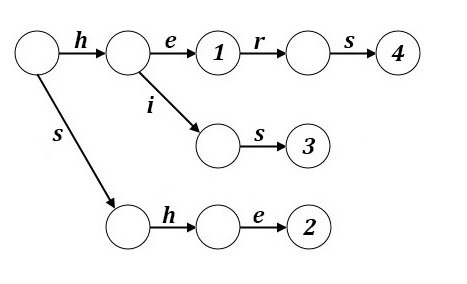
\includegraphics[width=0.5\linewidth]{/Users/daniilviner/Desktop/EDS-Study/2nd course/Algorithms/Бор.jpg}
\end{center}

\subsection{Суффиксные и автоматные ссылки}
Обозначим за $[u]$ слово, приводящее в вершину $u$ в боре

% \definition Суффиксная ссылка $l(v)$ ведёт в вершину $u \neq v$, которая соответствует наидлиннейшему принимаемому бором суффиксу $v$.

\definition Суффиксная ссылка $\pi(u)=v$, если $[v]$ — максимальный суффикс $[u]$, который одновременно является префиксом какого-то слова из словаря, при этом $[v]\ne[u]$

\definition Автоматный переход $\delta(v, c)$ ведёт в вершину, соответствующую максимальному принимаемому бором суффиксу строки $v + c$.

\subsubsection{Построение суффиксных ссылок}
\begin{minipage}{0.5\textwidth}
    Суффиксная ссылка для каждой вершины $u$ — это вершина, в которой оканчивается наидлиннейший собственный суффикс строки, соответствующей вершине $u$. Единственный особый случай — корень бора: для удобства суффиксную ссылку из него проведём в себя же.\\[2mm]
    Например, для вершины $5$ с соответствующей ей строкой $she$ максимальным подходящим суффиксом является строка $he$. Видим, что такая строка заканчивается в вершине $2$. Следовательно суффиксной ссылкой вершины для $5$ является вершина $2$
\end{minipage}
\begin{minipage}{0.5\textwidth}
    \begin{center}
        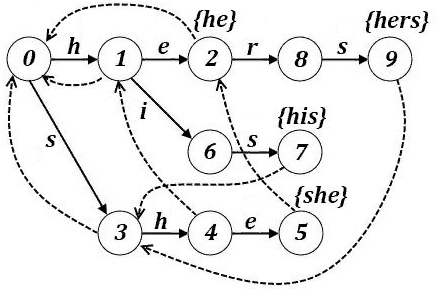
\includegraphics[width=0.9\linewidth]{/Users/daniilviner/Desktop/EDS-Study/2nd course/Algorithms/Axo.jpg}
    \end{center}
\end{minipage}

\subsubsection{Вычисление автоматных ссылок}
Автоматные ссылки вычисляются с использованием \textit{суффиксных ссылок} и обычных переходов. Алгоритм строит автоматные ссылки по следующей логике:
\begin{enumerate}
    \item Мы стоим в некоторой вершине $v$ и хотим перейти по символу $c$, тогда
    \begin{itemize}
        \item Если есть обычный переход по символу $c$, то автоматная ссылка просто указывает на этот переход: \code{v->autLink[c] = \&v->next[c]}
        \item Если из вершины $v$ нет перехода по $c$, то автоматная ссылка переходит по суффиксной ссылке (если ее нет, то автомат идет в корень)
        \begin{itemize}
            \item Смотрим, есть ли переход по символу $c$ из вершины, в которую мы попали
            \item Если да, то автоматная ссылка указывает на вершину, в которую мы попадем, сделав переход по $c$
            \item Если нет, то снова пытаемся пройти по суффиксной ссылке, повторяя алгоритм, пока не попадем либо в корень, либо к нужному ребру
        \end{itemize}
    \end{itemize}
%     \item Если символ $c$ существует в \code{v->next} (то есть есть обычный переход по символу $c$), то автоматная ссылка указывает на этот переход: \code{v->autLink[c] = \&v->next[c]}
%     \item Если символ $c$ не существует в \code{v->next}, то мы идем по суффиксной ссылке и смотрим, куда она ведет:
    \begin{itemize}
        \item Если текущая вершина — корень, то автоматная ссылка замыкается на сам корень, то есть: \code{v->autLink[c] = v}
        \item Если это не корень, то автоматная ссылка указывает на результат перехода по суффиксной ссылке: \code{v->autLink[c] = v->sufLink->autLink[c]}
     
    \end{itemize}
\end{enumerate}

\subsubsection{Работа автоматных ссылок и зачем они нужны}
Предположим, что мы находимся в вершине $v$ и хотим обработать символ $c$. Если в текущей вершине $v$ есть переход по символу $c$, то мы идем по обычному переходу (ребру), и всё продолжается как обычно.

Фактически, автоматная ссылка — это резервный переход в другую вершину, где мы можем продолжить поиск.

Автоматные ссылки помогают избежать возврата назад по тексту при поиске. Если символ не подошел, мы просто переходим к другой вершине, которая может соответствовать суффиксу уже обработанной части текста

\difficulty После построения автоматных ссылок мы можем переходить по ним за $O(1)$

\subsubsection{Сложность}
Пусть у нас есть словарь $s_1,s_2,\ldots,s_n$

Построение бора, суффиксных ссылок и автомата займет $O(m)$, где $m=\displaystyle\sum_{i=1}^{n} |s_i|$

\begin{enumerate}
    \item В боре каждая вершина соответствует одному символу из набора строк. Значит, мы добавляем каждый символ всех строк в бор один раз
    \item Суффиксные ссылки для каждой вершины бора строятся с помощью BFS. Для каждой вершины мы проверяем её суффиксную ссылку, а это делается за $O(m)$, так как каждая вершина обрабатывается один раз
    \item Автоматные ссылки тоже строятся в процессе обхода бора по тому же принципу, что и суффиксные ссылки. Для каждой вершины выполняется один проход по суффиксной ссылке и проверяются символы, что снова занимает $O(m)$ времени (построение)
\end{enumerate}

\newpage
\section{Суффиксный массив}
Суффиксным массивом строки $s$ называется перестановка индексов начал её суффиксов, которая задаёт порядок их лексикографической сортировки. Иными словами, чтобы его построить, нужно выполнить сортировку всех суффиксов заданной строки

\begin{center}
    \begin{tabular}{c l c l }
        % \hline
        \textbf{SA} & \textbf{} & \textbf{SA} & \textbf{} \\
        % \hline
        1  & mississippi\$  & 12 & \$ \\
        2  & ississippi\$   & 11 & i\$ \\
        3  & ssissippi\$    & 8  & ippi\$ \\
        4  & sissippi\$     & 5  & issippi\$ \\
        5  & issippi\$      & 2  & ississippi\$ \\
        6  & ssippi\$       & 1  & mississippi\$ \\
        7  & sippi\$        & 10 & pi\$ \\
        8  & ippi\$         & 9  & ppi\$ \\
        9  & ppi\$          & 7  & sippi\$ \\
        10 & pi\$           & 4  & sissippi\$ \\
        11 & i\$            & 6  & ssippi\$ \\
        12 & \$             & 3  & ssissippi\$ \\
        % \hline
    \end{tabular}

    Сортировка всех суффиксов строки <<mississippi\$>>
\end{center}

\subsection{Сортировка суффиксов}
Можно выделить три основных способа отсортировать суфмасс:
\begin{itemize}
    \item Пишем компаратор, который сравнивает все суффиксы, кидаем это в \code{std::sort}. Сложность —  $O(n^2\log n)$
    \item Используем хэшами, тогда асимптотика — $O(n\log^2 n)$
    \item Самый оптимальный метод — $O(n\log n)$
\end{itemize}

Рассмотрим самый оптимальный метод. В процессе мы будем использовать ранг суффикса — метка о лексикографическом порядке суффикса.
% Допишем в конец строки какой-нибудь символ, который лексикографически меньше любого другого, либо «\$», либо «\#», либо просто нулевой символ

% Мы будем выполнять сортировку не суффиксов, а \textit{циклических сдвигов}. Строки мы тоже будем рассматривать циклические — это удобно тем, что у них всех будет одна и та же длина.

% Алгоритм будет состоять из $\lceil \log n \rceil$ этапов. На $k$-том этапе будем сортировать все циклические подстроки длины $2^k$. Так на последнем этапе мы отсортируем строки длины $\geqslant n$ (это легально — строки ведь циклические), и мы получим нужный суффиксный массив.

% Заметим, что в отличие сортировки суффиксов, сортировка подстрок не всегда однозначна — две подстроки могут быть одинаковыми. Поэтому на каждой фазе алгоритма помимо перестановки $p$ индексов циклических подстрок мы должны поддерживать для каждой циклической подстроки номер её \textit{класса эквивалентности} $c_i$, которому эта подстрока принадлежит. Номера классов эквивалентности будем давать с сохранением порядка: лексикографически меньшим подстрокам соответствуют меньшие $c_i$. После последнего этапа массив классов эквивалентности должен задавать перестановку, обратную суффиксному массиву.
\begin{enumerate}
    \item Инициализация рангов
    \begin{itemize}
        \item Каждый суффикс строки сортируется по его первому символу. Это можно сделать с помощью сортирови подсчетом
        \item Каждый символ строки преобразуется в числовой ранг на основе его порядкового номера в алфавите
    \end{itemize}
    \item Итеративная сортировка по подстрокам длины $2^k$
    \begin{itemize}
        \item На каждом шаге мы удваиваем длину подстрок, по которым сортируем суффиксы
        \item Сначала сортируем по первым символам $(k = 1)$, затем по первым двум символам $(k = 2)$, четырём $(k = 4)$, и так далее, пока длина подстроки не станет больше длины строки
    \end{itemize}
    \item На каждом шаге сортировка суффиксов по подстрокам длины $2^k$ происходит в два этапа:
    \begin{itemize}
            \item Сортировка по первым k символам (используя ранги из предыдущего шага)
            \item Сортировка по следующим k символам (если они есть)
    \end{itemize}
    \item Обновление рангов
    \begin{itemize}
        \item После сортировки нужно обновить ранги суффиксов на основе их позиций в отсортированном массиве
        \item Если два суффикса равны по первым k символам, им присваивается одинаковый ранг. Если не равны, их ранги различаются
    \end{itemize}
\end{enumerate}

Процесс продолжается, пока длина подстрок, по которым происходит сортировка, не станет больше длины строки

\difficulty Этот алгоритм работает за $O(n \log n)$, где $n$ — длина строки, поскольку на каждом этапе сортировки подстрок мы используем сортировку подсчётом, которая работает за линейное время, и таких этапов будет примерно $\log n$, потому что мы каждый раз удваиваем длину строки

\subsection{Применение в задачах}
Суффиксный массив применяется в таких задачах, как
\begin{itemize}
    \item Поиск подстроки в строке
    \item Подсчет количества различных подстрок
    \item Нахождение LCP двух строк
\end{itemize}

\subsection{Поиск LCP. Алгоритм пяти корейцев}
Мы построили суффиксный массив, теперь попробуем найти LCP
\difficulty $O(n)$, где $n$ — длина строки

Алгоритм работает следующим образом
\begin{enumerate}
    \item Построение массива рангов:
    \begin{itemize}
        \item Для каждой позиции строки вычисляется её ранг, то есть позиция соответствующего суффикса в суффиксном массиве
        \item Пусть \code{rank[i]} — это индекс позиции $i$ в суффиксном массиве
    \end{itemize}
    \item Итерирование по суффиксам
    \begin{itemize}
        \item Для каждого суффикса строки на позиции $i$ мы пытаемся найти длину наибольшего общего префикса между суффиксом на позиции $i$ и суффиксом, который идёт перед ним в лексикографическом порядке
    \end{itemize}
    \item Если LCP для предыдущих суффиксов уже найден, можно использовать его для ускорения поиска. Мы знаем, что суффиксы уже совпадают на определённой длине и можем продолжать с этой длины)
\end{enumerate}

\begin{lstlisting}
    vector<int> calc_lcp(vector<int> &val, vector<int> &c, vector<int> &p) {
        int n = val.size();
        int l = 0;
        vector<int> lcp(n);
        for (int i = 0; i < n; i++) {
            if (c[i] == n - 1)
                continue;
            int nxt = p[c[i] + 1];
            while (max(i, nxt) + l < n && val[i + l] == val[nxt + l])
                l++;
            lcp[c[i]] = l;
            l = max(0, l - 1);
        }
        return lcp;
    }
\end{lstlisting}

\newpage
\section{Задача построения максимального потока в сети}
Задача заключается в том, чтобы найти максимальный поток, который можно провести из истока в сток через сеть, состоящую из вершин и ориентированных рёбер с заданными пропускными способностями

\begin{center}
    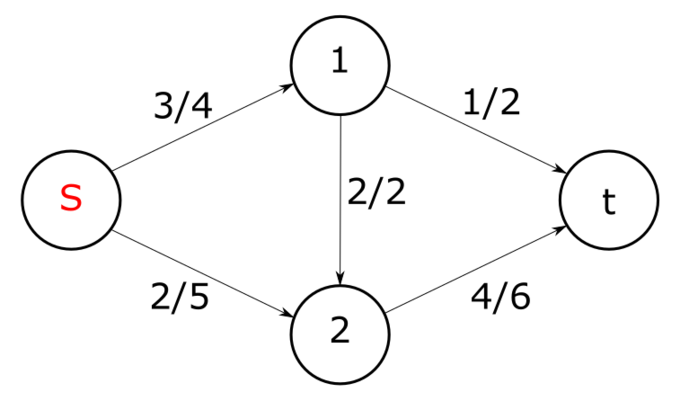
\includegraphics[width=0.5\linewidth]{/Users/daniilviner/Desktop/EDS-Study/2nd course/Algorithms/Сеть.png}
\end{center}
\subsection{Алгоритм Форда-Фалкерсона}
Алгоритм основан на методе поиска увеличивающих путей в сети

\definition \textit{Увеличивающий путь} — это путь от источника к стоку, по которому можно увеличить поток, не превышая пропускные способности рёбер

\begin{enumerate}
    \item Установить начальный поток в сети равным нулю
    \item Поиск увеличивающего пути
    \begin{itemize}
        \item Для этого можно использовать любой алгоритм поиска (DFS или BFS) для нахождения пути, где все рёбра имеют положительную остаточную пропускную способность
    \end{itemize}
    \item После нахождения увеличивающего пути определить минимальную остаточную пропускную способность по этому пути. Эта величина обозначает, насколько можно увеличить поток
    \item Увеличить поток
    \begin{itemize}
        \item Увеличить поток по всем рёбрам увеличивающего пути на значение минимальной остаточной пропускной способности
        \item Уменьшить остаточную пропускную способность по всем рёбрам пути на это значение
        \item Увеличить остаточную пропускную способность обратных рёбер (если поток проходит по ребру, создаётся обратное ребро, через которое поток может быть уменьшен в будущем)
    \end{itemize}
\end{enumerate}

Как только не удается найти увеличивающий путь, алгоритм завершает работу

% \comment Алгоритм не может работать с иррациональными числами, так как в таком случае всегда найдется некая малая величина, на которую можно будет увеличить поток
\difficulty $O(|E|f)$, где $E$ —  число рёбер в графе, $f$ — максимальный поток в графе, так как каждый увеличивающий путь может быть найден за $O(E)$ и увеличивает поток как минимум на $1$

\subsection{Минимальный разрез сети}
\definition \textit{Минимальный разрез сети} — это  разделение графа на две части (одна часть содержит исток, другая — сток), которое минимизирует сумму пропускных способностей рёбер, пересекающих разрез в одном направлении

\comment Величина максимального потока равна пропускной способности минимального разреза

\subsection{Алгоритм Эдмондса-Карпа}
Алгоритм Эдмонса-Карпа — это улучшение алгоритма Форда-Фалкерсона, которое использует поиск в ширину (BFS) для нахождения увеличивающих путей в графе. Этот алгоритм решает задачу нахождения максимального потока в сети с гораздо более предсказуемым временем работы, чем оригинальный алгоритм Форда-Фалкерсона

\begin{enumerate}
    \item Положим все потоки равными нулю. Остаточная сеть изначально совпадает с исходной сетью
    \item В остаточной сети находим кратчайший путь из источника в сток. Если такого пути нет, останавливаемся
    \item Пускаем через найденный путь (он называется увеличивающим путём или увеличивающей цепью) максимально возможный поток
    \begin{itemize}
        \item На найденном пути в остаточной сети ищем ребро с минимальной пропускной способностью $c_{\min}$
        \item Для каждого ребра на найденном пути увеличиваем поток на $c_{\min}$, а в противоположном ему — уменьшаем на $c_{\min}$
        \item Модифицируем остаточную сеть. Для всех рёбер на найденном пути, а также для противоположных им рёбер, вычисляем новую пропускную способность. Если она стала ненулевой, добавляем ребро к остаточной сети, а если обнулилась, стираем его
    \end{itemize}
\end{enumerate}

\difficulty $O(VE^2)$, где $V$ — количество вершин в графе, а $E$ — количество рёбер 
% Это связано с тем, что каждый путь увеличивает поток, а минимальное количество рёбер (по числу) на пути минимизирует количество изменений в остаточной сети.


\newpage
\section{Максимальное паросочетание в двудольном графе}
В задаче поиска максимального паросочетания в графе требуется найти наибольший набор рёбер, не имеющих общих вершин

\definition \textit{Паросочетание} — это набор рёбер, не имеющих общих вершин, то есть никакие два ребра не должны делить вершину

\subsection{Алгоритм Куна}
Начнем с пустого паросочетания и будем искать увеличивающие цепи, пока они ищутся
\begin{enumerate}
    \item Для каждой вершины из множества $U$ пытаемся найти её пару из множества $V$
    \item Ищем увеличивающие пути
    \begin{itemize}
        \item Для каждой вершины \( u \in U \) проверяем, можно ли её присоединить к какому-то элементу из множества \( V \). Используем для этого DFS
        \item Если вершина не используется в другом паросочетании, то соединяем, если используется, запускаем DFS для вершины из $V$ и пытаемся присоединить к другой вершине
        \item Если удаётся найти увеличивающий путь (путь, по которому можно провести обмен, чтобы увеличить паросочетание), то обновляем текущее паросочетание
    \end{itemize}
    \item Каждый раз, когда находим увеличивающий путь, добавляем его в текущее паросочетание и пересчитываем.
\end{enumerate}

\difficulty \( O(VE) \), где \( E \) — количество рёбер, а \( V \) — количество вершин

\newpage
\section{Деревья поиска}
\textbf{\textit{Бинарное дерево поиска}} — дерево, для которого выполняются следующие свойства:
\begin{itemize}
\item У каждой вершины не более двух детей
\item Все вершины обладают \textit{ключами}, на которых определена операция сравнения (например, целые числа или строки)
\item У всех вершин \textit{левого} поддерева вершины $v$ ключи \textit{не больше}, чем ключ $v$
\item У всех вершин \textit{правого} поддерева вершины $v$ ключи \textit{больше}, чем ключ $v$
\item Оба поддерева — левое и правое — являются двоичными деревьями поиска
\end{itemize}
В \textit{небинарных} деревьях количество детей может быть больше двух, и при этом в «более левых» поддеревьях ключи должны быть меньше, чем «более правых»\\[2mm]
\indent Для работы с деревьями поиска нужно создать структуру
\begin{lstlisting}
struct Node:
  T key                    // key of the node
  Node left                // pointer to the left child
  Node right               // pointer to the right child
  Node parent              // pointer to the parent
\end{lstlisting}
\subsection{Поиск элемента}
Нужна функция, прнимающая корень дерева и искомый ключ
\begin{itemize}
    \item Для каждого узла сравниваем значение его ключа с искомым ключом
    \item Если ключи одинаковы, то функция возвращает текущий узел
    \item В противном случае функция вызывается рекурсивно для левого или правого поддерева
\end{itemize}
% \begin{lstlisting}
% Node search(x : Node, k : T):
%    if x == null or k == x.key
%       return x
%    if k < x.key
%       return search(x.left, k)
%    else
%       return search(x.right, k)
% \end{lstlisting}
\textbf{Сложность в худшем случае} — $O(h)$ ($h$ — высота дерева), так как узлы, которые посещает функция образуют нисходящее дерево. Такое возможно, когда дерево является «бамбуком»\\[2mm]
\textbf{Сложность при оптимизации} — $O(\log N)$. Если изменить способ хранения дерева, например сразу при проходе до какого-то ключа записать его как ключ ко всем вершинам в пути, то сложность снизится

\subsection{Вставка элемента}
Почти то же самое, что поиск элемента, но теперь при обнаружении у элемента отсутствия ребенка нужно подвесить на него вставляемый элемент
\begin{lstlisting}
Node insert(x : Node, z : T):               // x - root of the subtree, z - key to be inserted
   if x == null 
      return Node(z)                        // attach a Node with key = z
   else if z < x.key
      x.left = insert(x.left, z)
   else if z > x.key
      x.right = insert(x.right, z)
   return x
\end{lstlisting}

\subsection{Удаление элемента}
Рассмотрим три случая при рекурсивной реализации
\begin{enumerate}
    \item Удаляемый элемент находится в \textit{левом} поддереве текущего поддерева
    \begin{itemize}
        \item тогда нужно рекурсивно удалить элемент из нужного поддерева
    \end{itemize}
    \item Удаляемый элемент находится в \textit{правом} поддереве
    \begin{itemize}
        \item тогда нужно рекурсивно удалить элемент из нужного поддерева
    \end{itemize}
    \item Удаляемый элемент находится в \textit{корне}, то два случая:
    \begin{itemize}
        \item имеет два дочерних узла
        \begin{itemize}
            \item нужно заменить его минимальным элементом из правого поддерева и рекурсивно удалить этот минимальный элемент из правого поддерева
        \end{itemize}
        \item имеет один дочерний узел
        \begin{itemize}
            \item нужно заменить удаляемый элемент потомком
        \end{itemize}
    \end{itemize}
\end{enumerate}
% \begin{lstlisting}
% Node delete(root : Node, z : T):    // root of subtree, key to delete
%   if root == null
%     return root
%   if z < root.key
%     root.left = delete(root.left, z)
%   else if z > root.key
%     root.right = delete(root.right, z)
%   else if root.left != null and root.right != null
%     root.key = minimum(root.right).key
%     root.right = delete(root.right, root.key)
%   else
%     if root.left != null
%       root = root.left
%     else if root.right != null
%       root = root.right
%     else
%       root = null
%   return root
% \end{lstlisting}
% \subsubsection*{Еще один вариант объяснения}
% \begin{enumerate}
%     \item Если пытаемся удалить лист или какую-то вершину в одном из поддеревьев, то все хорошо. Просто вырезаем вершину и на ее место ставим потомка и всех потомков потомка
%     \item Если же пытаемся удалить 
% \end{enumerate}

\subsection{AVL-деревья}
\definition \textit{AVL-дерево} — сбалансированное двоичное дерево поиска, в котором поддерживается следующее свойство: для каждой его вершины высота её двух поддеревьев различается не более чем на 1

\definition \textit{Баланс дерева} — это разница между высотой левого и правого поддерева

\subsection{Добавление элемента и балансировка AVL-дерева}

\begin{enumerate}
    \item \textbf{Добавление элемента}
    \begin{itemize}
        \item Используем стандартный алгоритм добавления в бинарное дерево поиска (BST). Сравниваем значение добавляемого элемента с текущим узлом:
        \begin{itemize}
            \item Если значение меньше текущего, переходим к левому поддереву.
            \item Если больше — к правому.
        \end{itemize}
        \item После нахождения подходящей позиции вставляем новый узел.
    \end{itemize}

    \item \textbf{Обновление высот}
    \begin{itemize}
        \item После добавления узла необходимо обновить высоты всех предков вставленного узла. Для каждого узла, начиная с родителя вставленного узла до корня, вычисляем новую высоту как \code{1 + max(\text{height(left)}, \text{height(right)})}
    \end{itemize}

    \item \textbf{Проверка баланса}
    \begin{itemize}
        \item Для каждого узла, начиная с родителя вставленного узла, проверяем его баланс:
        \item Если баланс узла стал равен $2$ или $-2$, значит, дерево стало несбалансированным, и нужно выполнить ротации.
    \end{itemize}

    \item \textbf{Повороты}
    \begin{itemize}
        \item \textbf{LL-rotation (Правый поворот):} Если баланс $2$, а добавление произошло в левое поддерево левого дочернего узла.
        \item \textbf{RR-rotation (Левый поворот):} Если баланс $-2$, а добавление произошло в правое поддерево правого дочернего узла.
        \item \textbf{LR-rotation (Левый-правый поворот):} Если баланс $2$, а добавление произошло в правое поддерево левого дочернего узла. Сначала выполняем левый поворот на левом дочернем узле, затем правый поворот на текущем узле.
        \item \textbf{RL-rotation (Правый-левый поворот):} Если баланс $-2$, а добавление произошло в левое поддерево правого дочернего узла. Сначала выполняем правый поворот на правом дочернем узле, затем левый поворот на текущем узле.
    \end{itemize}
\end{enumerate}

\subsection{Высота AVL-дерева}
AVL-дерево с $n$ ключами имеет высоту $O(\log n)$


























\end{document}